\documentclass[12pt,a4paper]{article}
\usepackage[a4paper, margin=2cm]{geometry}
\usepackage{iftex}
\ifPDFTeX
  \usepackage[T5]{fontenc}
  \usepackage[utf8]{inputenc}
  \usepackage[vietnamese]{babel}
\else
  \usepackage{fontspec}
  \usepackage[vietnamese]{babel}
\fi
\usepackage{amsmath,amssymb,amsthm}
\usepackage{graphicx}
\usepackage[export]{adjustbox}
\usepackage{algorithm}
\usepackage{algpseudocode}
\usepackage{booktabs}
\usepackage{tabularx}
\usepackage{float}
\usepackage{xcolor}
\usepackage{listings}
\usepackage[hidelinks]{hyperref}

\floatname{algorithm}{Thuật toán}
\renewcommand{\algorithmicrequire}{\textbf{Input:}}
\renewcommand{\algorithmicensure}{\textbf{Output:}}
\newcommand{\todo}[1]{\textcolor{red}{\textbf{[#1]}}}
\lstset{basicstyle=\ttfamily\small, breaklines=true, frame=single, columns=fullflexible, keepspaces=true}

\begin{document}

\begin{center}
    \textbf{TRƯỜNG ĐẠI HỌC CNTT - ĐHQG TP.HCM} \\
    \textbf{KHOA KHOA HỌC MÁY TÍNH} \\
    \vspace{1.5cm}
    \textbf{Môn học} \\
    \textbf{Phân tích và thiết kế thuật toán} \\
    \textbf{(Design and Analysis of Algorithms)} \\
    \vspace{1.5cm}
    {\Large \textbf{BÀI TẬP LỚN}} \\[4pt]
    {\large \textbf{Trực quan hóa thuật toán Quay lui giải bài toán Địa chỉ IP (WeCode)}}
\end{center}

\vfill
\noindent
\textbf{Assignment:} Bài tập lớn \\
\textbf{Họ và Tên:} Đỗ Quốc Học \\
\textbf{MSSV:} 26410045 \\
\textbf{Ngày nộp bài:} 07/10/2026

\newpage
\tableofcontents
\newpage

%=====================================================================
\section{Sản phẩm nộp}

\begin{enumerate}
    \item \textbf{Source code:} thư mục \texttt{source/}
    \begin{itemize}
        \item \texttt{index.html} --- ứng dụng web trực quan hóa (mở trực tiếp bằng trình duyệt, không cần cài đặt).
        \item \texttt{ip\_wecode.py} --- lời giải Python (quay lui) dùng để nộp WeCode.
        \item \texttt{ip\_bruteforce.py} --- bản vét cạn độc lập, dùng làm đáp án đối chứng.
        \item \texttt{gen\_testcases.py}, \texttt{embed\_tests.py}, \texttt{test\_core.js} --- sinh testcase, nhúng vào trang và kiểm thử lõi thuật toán.
    \end{itemize}
    \item \textbf{Video demo:} \texttt{demo/demo\_video.mp4} (3 phút 9 giây, $11$ cảnh, có giọng đọc và phụ đề). Video được nén cùng toàn bộ sản phẩm thành một tệp \texttt{.rar} và nộp qua đường dẫn của cô.
    \item \textbf{Bộ testcase:} thư mục \texttt{testcases/} (48 cặp \texttt{.in}/\texttt{.out}, \texttt{tests.json}, \texttt{README.md}).
    \item \textbf{Báo cáo:} tài liệu này (\texttt{report/}).
\end{enumerate}

%=====================================================================
\section{Giới thiệu bài toán}

\textbf{Lý do chọn.} Bài ``Địa chỉ IP'' có liên quan trực tiếp đến công việc của em, nên em nắm rõ ngữ cảnh sử dụng của bài toán và đánh giá được kết quả của ứng dụng có hợp lý hay không. Đây cũng là bài em đã làm ở Lab\#01 (Backtracking) trên WeCode, nay chọn lại làm bài tập lớn cuối kì, nên em đã nắm rõ đề và tập trung vào phần trực quan hóa và kiểm thử. Về mặt thuật toán, bài thuộc Lab\#01, đề ghi rõ phải dùng quay lui, kỹ thuật khác thì giảng viên không chấm. Bài có không gian trạng thái nhỏ và có cấu trúc rõ (bốn đoạn, mỗi đoạn một đến ba chữ số), nên cây quay lui đủ nhỏ để vẽ ra và theo dõi từng bước, nhưng vẫn có đủ hai loại loại bỏ nhánh khác nhau (loại ứng viên sai và cắt tỉa theo độ dài). Đây là điều em cần để so sánh ``quay lui có và không cắt tỉa'' với ``vét cạn''.

\textbf{Nguồn gốc và phần tham khảo.} Tên bài, yêu cầu dùng quay lui và ví dụ \texttt{25525511135} lấy từ đề của môn trên WeCode (Lab\#01), do em cung cấp cho AI dưới dạng ảnh chụp đề. Các phần còn lại \textbf{không có trong phần đề được cung cấp}, mà AI (Claude Sonnet 5.5) dựa vào kiến thức có sẵn để xây dựng: luật của một địa chỉ IPv4 (bốn đoạn, giá trị $0$ đến $255$, không số $0$ đứng đầu), khung thuật toán quay lui, kỹ thuật cắt tỉa theo độ dài còn lại, thứ tự thử độ dài $1,2,3$. Bài này cùng dạng với bài ``Restore IP Addresses'' (LeetCode 93). Để không chỉ dựa vào trí nhớ của AI, các điểm trên được đối chiếu lại với các nguồn ở mục \ref{sec:refs}, ghi rõ điều gì nguồn xác nhận và điều gì không.

\textbf{Ứng dụng thực tế.} Khôi phục dữ liệu bị mất ký tự phân cách (log mạng, văn bản OCR, tệp cấu hình hỏng), và là ví dụ điển hình của dạng ``chia chuỗi thành các phần thỏa ràng buộc'' trong phân tích cú pháp.

%=====================================================================
\section{Mô tả bài toán}

Bạn Bình cấu hình mạng cho một tiệm net. Do phần mềm gõ văn bản gặp lỗi, mọi dấu chấm trong các địa chỉ IP bị mất. Cho chuỗi $s$ chỉ gồm các chữ số, hãy liệt kê mọi địa chỉ IPv4 hợp lệ có thể có bằng cách chèn đúng ba dấu chấm vào $s$.

\textbf{Giả định về luật địa chỉ IP.} Phần đề được cung cấp cho AI chỉ nói ``các địa chỉ IP có thể có'', không liệt kê điều kiện của từng đoạn. Em áp dụng luật chuẩn của IPv4: bốn đoạn, giá trị từ $0$ đến $255$, không có số $0$ đứng đầu (trừ chính số $0$). Ví dụ của đề (\texttt{25525511135} cho đúng hai địa chỉ) khớp với luật này, nhưng đề không nêu luật thành lời, nên coi đây là giả định chuẩn và đã đối chiếu nguồn ở mục~\ref{sec:refs}.

%=====================================================================
\section{Mô hình bài toán}\label{sec:model}

\subsection{Input, Output}
\begin{itemize}
    \item \textbf{Input:} chuỗi $s$ ($|s| = n$), kiểu \texttt{string}, giới hạn $1 \le n \le 100$ theo đề (``không quá 100 ký tự''), mỗi ký tự $s_i \in \{0, 1, \dots, 9\}$.
    \item \textbf{Output:} tập $R$ gồm mọi địa chỉ IP $a_1.a_2.a_3.a_4$ thỏa các ràng buộc dưới đây, mỗi địa chỉ một dòng, thứ tự tùy ý. Nếu $R = \emptyset$ thì không in gì.
\end{itemize}

\subsection{Ràng buộc}
Địa chỉ $a_1.a_2.a_3.a_4$ hợp lệ khi và chỉ khi:
\begin{enumerate}
    \item $a_1 a_2 a_3 a_4 = s$ (ghép bốn đoạn theo thứ tự ra đúng chuỗi $s$, dùng hết ký tự);
    \item $1 \le |a_k| \le 3$ với mọi $k$;
    \item $0 \le \operatorname{int}(a_k) \le 255$;
    \item $a_k$ không có số $0$ đứng đầu, trừ khi $a_k = \text{``0''}$.
\end{enumerate}

\subsection{Ví dụ}
\begin{table}[H]
\centering
\begin{tabular}{@{}lll@{}}
\toprule
\textbf{Input} & \textbf{Output} & \textbf{Ghi chú} \\
\midrule
\texttt{25525511135} & \texttt{255.255.11.135}, \texttt{255.255.111.35} & ví dụ của đề \\
\texttt{010010} & \texttt{0.10.0.10}, \texttt{0.100.1.0} & số $0$ đứng đầu \\
\texttt{0000} & \texttt{0.0.0.0} & chỉ một cách \\
\texttt{123} & (không có) & ngắn hơn 4 ký tự \\
\texttt{256256256256} & (không có) & mọi đoạn $>255$ \\
\bottomrule
\end{tabular}
\end{table}

%=====================================================================
\section{Thiết kế cấu trúc dữ liệu và thuật toán}\label{sec:algo}

\subsection{Cấu trúc dữ liệu}
\begin{itemize}
    \item \texttt{s}: chuỗi đầu vào, \texttt{n = |s|}.
    \item \texttt{parts}: ngăn xếp (stack) các đoạn đã chọn, tối đa $4$ phần tử. Chiều dài \texttt{parts} chính là $k$, số đoạn đã chọn.
    \item \texttt{pos}: vị trí ký tự kế tiếp chưa dùng trong $s$.
    \item \texttt{out}: danh sách kết quả.
    \item (Chỉ có trong ứng dụng) \texttt{tree}: mảng nút của cây quay lui, mỗi nút lưu cha, đoạn đã chọn, độ sâu và trạng thái (đang thử, hợp lệ, bị loại, bị tỉa, là nghiệm).
\end{itemize}

\subsection{Phân tích đặc trưng và ý tưởng}
Một nghiệm là một cách chọn $3$ vị trí cắt trong $n-1$ khe giữa các ký tự. Mỗi đoạn chỉ có $3$ độ dài khả dĩ, nên cây quyết định có độ sâu tối đa $4$ và nhân tố rẽ nhánh tối đa $3$, tức không quá $3^4 = 81$ lá, bất kể $n$.
Hai nhận xét cho phép loại nhánh sớm:
\begin{enumerate}
    \item \textbf{Loại ứng viên.} Nếu đoạn $\operatorname{seg}$ dài hơn $1$ ký tự mà bắt đầu bằng \texttt{'0'}, hoặc $\operatorname{int}(\operatorname{seg}) > 255$, thì loại. Hơn nữa mọi đoạn \emph{dài hơn} bắt đầu từ cùng vị trí cũng sai (vẫn bắt đầu bằng \texttt{'0'}, hoặc là số lớn hơn), nên được phép \texttt{break} cả vòng lặp độ dài.
    \item \textbf{Cắt tỉa theo độ dài còn lại.} Đã chọn $k$ đoạn, còn $\ell = n - \text{pos}$ ký tự và cần $4-k$ đoạn nữa. Cần $\ell \ge 4-k$ (mỗi đoạn ít nhất $1$ ký tự) và $\ell \le 3(4-k)$ (mỗi đoạn nhiều nhất $3$ ký tự). Vi phạm một trong hai thì không thể ra nghiệm.
\end{enumerate}

\subsection{Mã giả}
\begin{algorithm}[H]
\caption{\textsc{Backtrack}(pos, parts)}
\begin{algorithmic}[1]
\Require chuỗi $s$ ($n = |s|$), vị trí $pos$, ngăn xếp $parts$
\Ensure ghi vào $out$ mọi địa chỉ hợp lệ có tiền tố $parts$
\State $k \gets |parts|$; \quad $\ell \gets n - pos$
\If{$\ell < 4-k$ \textbf{or} $\ell > 3(4-k)$} \Return \Comment{cắt tỉa theo độ dài}
\EndIf
\If{$k = 4$}
    \If{$pos = n$} thêm \texttt{join(parts, '.')} vào $out$ \EndIf
    \State \Return
\EndIf
\For{$len \gets 1$ \textbf{to} $3$}
    \If{$pos + len > n$} \textbf{break} \EndIf
    \State $seg \gets s[pos \,..\, pos+len)$
    \If{$len > 1$ \textbf{and} $seg[0] = \texttt{'0'}$} \textbf{break} \EndIf
    \If{$\operatorname{int}(seg) > 255$} \textbf{break} \EndIf
    \State $parts.\text{push}(seg)$
    \State \Call{Backtrack}{$pos + len$, $parts$}
    \State $parts.\text{pop}()$
\EndFor
\end{algorithmic}
\end{algorithm}
Gọi \textsc{Backtrack}(0, []). Mã nguồn tương ứng nằm ở \texttt{source/ip\_wecode.py} (hàm \texttt{bt}).

\subsection{Tính đúng đắn}
\emph{An toàn (không bỏ sót nghiệm).} Cả ba chỗ loại bỏ đều chỉ loại những lựa chọn chắc chắn không thể dẫn tới nghiệm: đoạn có số $0$ đầu, đoạn $>255$ (và các đoạn dài hơn, như đã chứng minh ở trên), và tình huống độ dài còn lại không chia nổi cho số đoạn còn lại. \emph{Đầy đủ (không sinh nghiệm sai).} Nghiệm chỉ được ghi khi $k=4$ và $pos=n$, mỗi đoạn đã qua kiểm tra. \emph{Không trùng.} Hai đường đi khác nhau trên cây có dãy độ dài đoạn khác nhau, tức vị trí chấm khác nhau, nên cho hai chuỗi khác nhau.

\subsection{Độ phức tạp}
Cây có độ sâu $\le 4$, mỗi nút có $\le 3$ con, nên số nút $\le 1 + 3 + 9 + 27 + 81 = 121$. Số này khớp với đo đạc: với chuỗi dài, quay lui không cắt tỉa thử đúng $120$ đoạn (cột ``QL không tỉa'' của bảng \ref{tab:cmp}), tức $121$ nút trừ nút gốc. Mỗi nút tốn $O(1)$ (đoạn dài tối đa $3$ ký tự), cộng thêm $O(n)$ để ghép mỗi nghiệm. Vậy \textbf{thời gian $O(3^4 + |R| \cdot n) = O(n)$ theo $n$}, tức hằng số theo bài toán này, và bộ nhớ $O(n)$.

Với vét cạn, số cách chọn $3$ vị trí cắt là $\binom{n-1}{3} = \Theta(n^3)$, tức $156\,849$ cách khi $n=100$. Quay lui có cắt tỉa gặp chuỗi quá dài thì dừng ngay tại gốc ($1$ nút).

%=====================================================================
\section{Ví dụ minh họa các bước thực hiện}\label{sec:example}

Xét $s = \texttt{25525511135}$ ($n=11$). Đây là cây quay lui thật do ứng dụng sinh ra (xuất từ \texttt{runAll}), $21$ nút kể cả gốc, trạng thái tỉa độ dài bật.

Mỗi dòng dưới đây ghi $k$ (số đoạn đã chọn sau khi thêm đoạn này), $\ell$ (số ký tự còn lại) và khoảng $\ell$ cần có để còn khả năng ra nghiệm, $[4-k,\ 3(4-k)]$. Dữ liệu lấy trực tiếp từ cây do ứng dụng sinh ra.

\begin{table}[H]
\centering
\scriptsize
\begin{tabular}{@{}rlllcp{4.4cm}@{}}
\toprule
\textbf{Nút} & \textbf{Đường đi} & \textbf{Trạng thái} & $k$, $\ell$ & \textbf{Cần $\ell\in$} & \textbf{Lý do} \\
\midrule
1  & \texttt{2}                 & tỉa            & 1, 10 & [3, 9] & $10 > 9$ \\
2  & \texttt{25}                & hết nhánh con  & 1, 9  & [3, 9] & hợp lệ, các con đều tỉa hoặc loại \\
3  & \texttt{25.5}              & tỉa            & 2, 8  & [2, 6] & $8 > 6$ \\
4  & \texttt{25.52}             & tỉa            & 2, 7  & [2, 6] & $7 > 6$ \\
5  & \texttt{25.525}            & loại           & 2, 6  & ---    & $525 > 255$ \\
6  & \texttt{255}               & có nghiệm      & 1, 8  & [3, 9] & hợp lệ \\
7  & \texttt{255.2}             & tỉa            & 2, 7  & [2, 6] & $7 > 6$ \\
8  & \texttt{255.25}            & hết nhánh con  & 2, 6  & [2, 6] & hợp lệ, các con đều tỉa hoặc loại \\
9  & \texttt{255.25.5}          & tỉa            & 3, 5  & [1, 3] & $5 > 3$ \\
10 & \texttt{255.25.51}         & tỉa            & 3, 4  & [1, 3] & $4 > 3$ \\
11 & \texttt{255.25.511}        & loại           & 3, 3  & ---    & $511 > 255$ \\
12 & \texttt{255.255}           & có nghiệm      & 2, 5  & [2, 6] & hợp lệ \\
13 & \texttt{255.255.1}         & tỉa            & 3, 4  & [1, 3] & $4 > 3$ \\
14 & \texttt{255.255.11}        & có nghiệm      & 3, 3  & [1, 3] & hợp lệ \\
15 & \texttt{255.255.11.1}      & tỉa            & 4, 2  & [0, 0] & còn dư $2$ ký tự \\
16 & \texttt{255.255.11.13}     & tỉa            & 4, 1  & [0, 0] & còn dư $1$ ký tự \\
17 & \texttt{255.255.11.135}    & \textbf{nghiệm} & 4, 0 & [0, 0] & dùng hết chuỗi \\
18 & \texttt{255.255.111}       & có nghiệm      & 3, 2  & [1, 3] & hợp lệ \\
19 & \texttt{255.255.111.3}     & tỉa            & 4, 1  & [0, 0] & còn dư $1$ ký tự \\
20 & \texttt{255.255.111.35}    & \textbf{nghiệm} & 4, 0 & [0, 0] & dùng hết chuỗi \\
\bottomrule
\end{tabular}
\end{table}

Chú thích: ``tỉa'' là bị cắt ngay đầu lần gọi đệ quy của nút đó bởi điều kiện độ dài. ``Hết nhánh con'' là nút hợp lệ nhưng mọi nút con của nó đều bị tỉa hoặc loại, nên không dẫn tới nghiệm.

Tổng hợp số liệu của lần chạy này (khớp với bảng thống kê trên giao diện): \textbf{19 nút được duyệt, 20 đoạn đã thử, 2 đoạn bị loại, 10 nhánh bị tỉa, 2 địa chỉ}.

\begin{figure}[H]
\centering
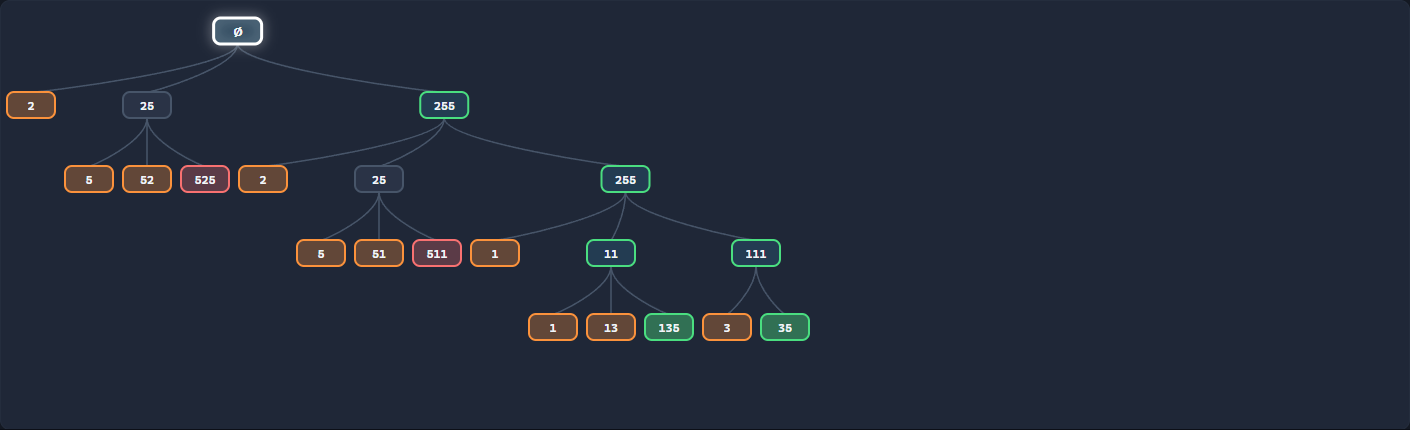
\includegraphics[width=\textwidth]{img/03_tree_sample.png}
\caption{Cây quay lui của \texttt{25525511135}. Cam: tỉa theo độ dài. Đỏ: loại ($>255$ hoặc $0$ đầu). Xanh lá: nghiệm hoặc nhánh có nghiệm.}
\end{figure}

%=====================================================================
\section{Thiết kế và xây dựng ứng dụng}

\subsection{Công nghệ}
Một tệp \texttt{index.html} duy nhất (HTML, CSS, JavaScript thuần), mở bằng trình duyệt là chạy. Thuật toán viết bằng \textbf{generator} \texttt{function*}: mỗi \texttt{yield} là một sự kiện (vào nút, thử đoạn, loại, tỉa, nhận nghiệm, quay lui). Nhờ vậy ứng dụng chạy từng bước, tạm dừng, chỉnh tốc độ mà không treo giao diện. Cây vẽ bằng SVG, tô lại sau mỗi sự kiện.

\subsection{Chức năng}
\begin{enumerate}
    \item \textbf{Nhập input} có kiểm tra: rỗng, có ký tự không phải số, dài hơn $100$ đều báo lỗi và khóa nút giải (hình \ref{fig:invalid}).
    \item \textbf{Chạy tự động / từng bước / làm lại}, thanh trượt tốc độ.
    \item \textbf{Dải chữ số} tô màu theo bốn đoạn đã chọn, đoạn đang thử tô vàng (đỏ nếu bị loại).
    \item \textbf{Mã giả} có dòng đang thực thi được tô sáng, đối chiếu từng bước với mã giả ở mục~\ref{sec:algo}.
    \item \textbf{Nhật ký} mỗi bước một dòng, ghi lý do.
    \item \textbf{Cây quay lui} vẽ theo thời gian thực, đổi màu theo trạng thái nút.
    \item \textbf{Bảng thống kê}: số nút duyệt, đoạn đã thử, đoạn bị loại, nhánh bị tỉa, số IP, số cách cắt của vét cạn.
    \item \textbf{Công tắc cắt tỉa theo độ dài} để thấy cây thay đổi thế nào.
    \item \textbf{So sánh ba cách} trên cùng một chuỗi: vét cạn, quay lui không tỉa, quay lui có tỉa (mục~\ref{sec:compare}).
    \item \textbf{Chạy toàn bộ testcase} ngay trong trang, so với đáp án nhúng sẵn.
    \item \textbf{Sinh chuỗi ngẫu nhiên có nghiệm} và các test mẫu chọn nhanh.
\end{enumerate}

\begin{figure}[H]
\centering
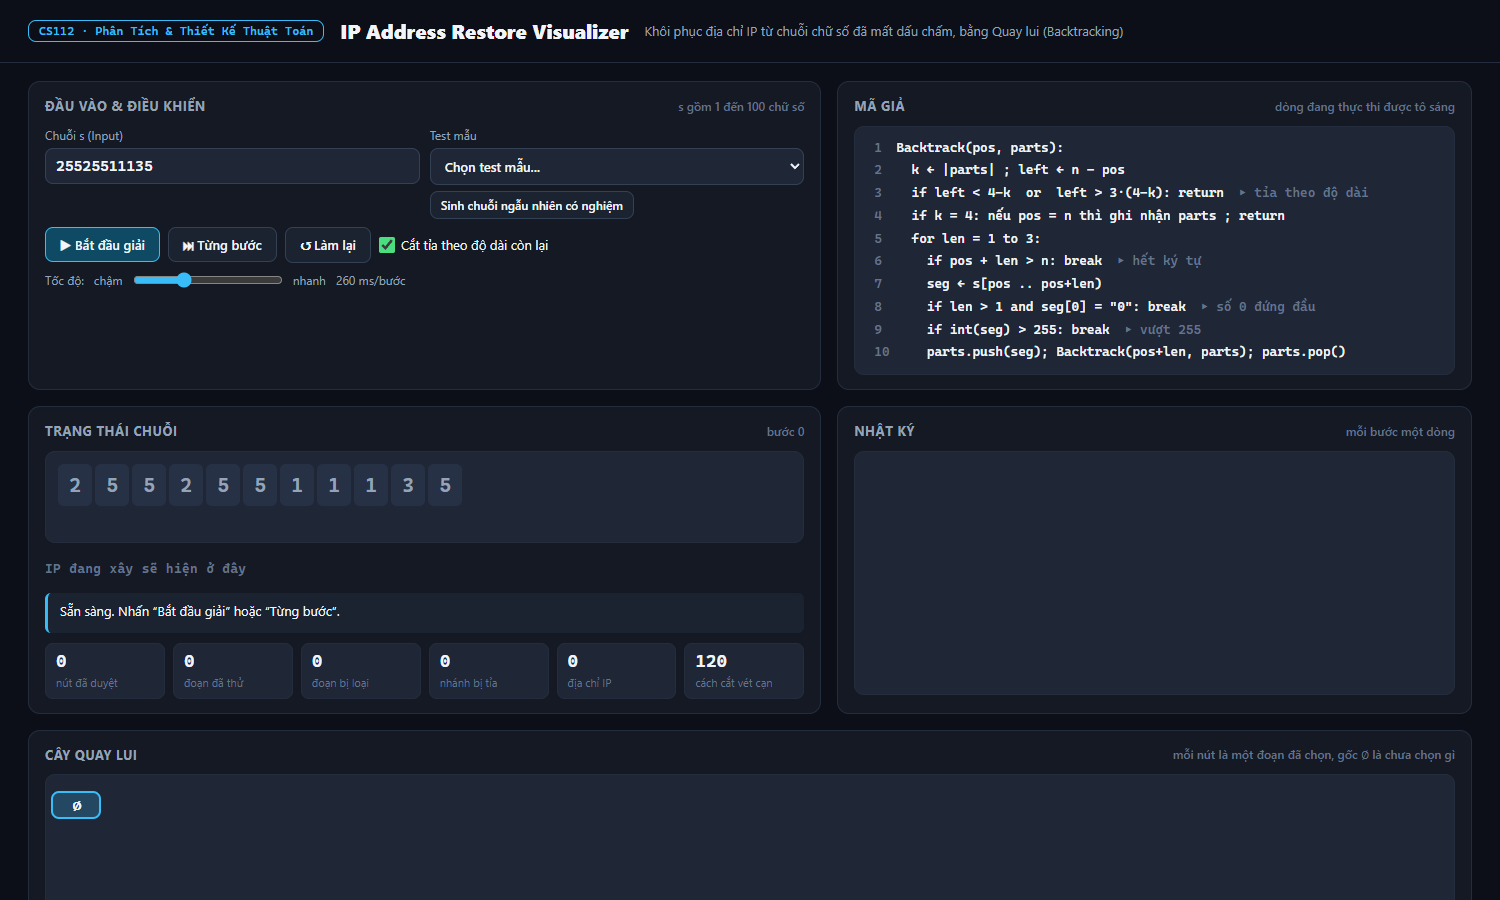
\includegraphics[width=\textwidth]{img/01_overview.png}
\caption{Giao diện tổng quan.}
\end{figure}
\begin{figure}[H]
\centering
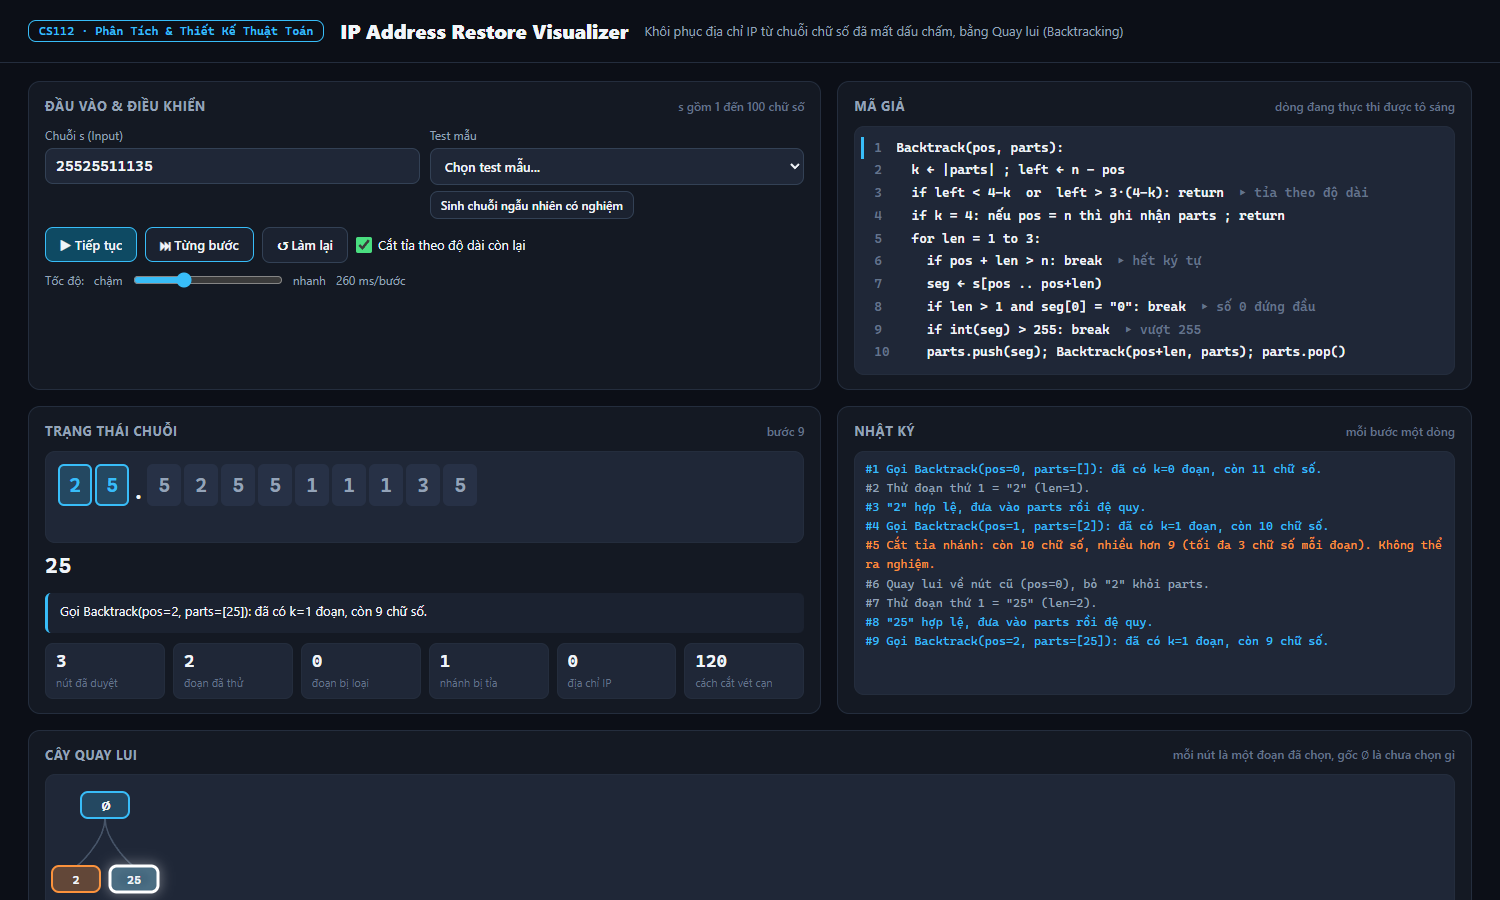
\includegraphics[width=\textwidth]{img/02_step_mode.png}
\caption{Chế độ từng bước: dải chữ số tô màu, dòng mã giả đang chạy, nhật ký.}
\end{figure}
\begin{figure}[H]
\centering
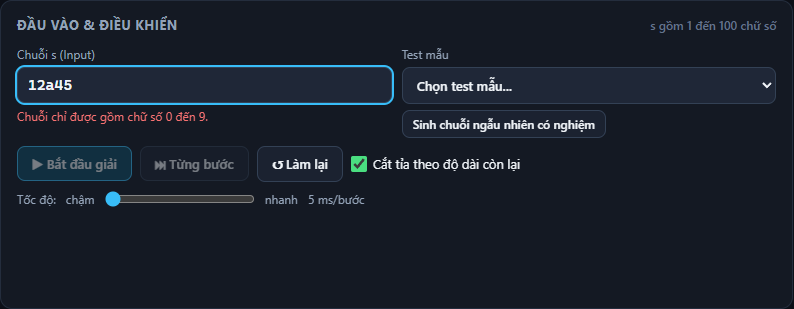
\includegraphics[width=0.9\textwidth]{img/07_invalid_input.png}
\caption{Nhập chuỗi có chữ cái: báo lỗi và khóa nút giải.}\label{fig:invalid}
\end{figure}

\subsection{Hướng dẫn sử dụng bảng điều khiển (dashboard)}\label{sec:guide}

\textbf{Cách mở ứng dụng (Windows).} Ứng dụng chỉ là một trang web nằm trong một tệp duy nhất, không cần cài đặt gì, không cần Internet.
\begin{enumerate}
    \item Giải nén tệp \texttt{.rar} đã nộp (nhấp chuột phải vào tệp, chọn \emph{Extract Here} hoặc \emph{Giải nén vào đây}). Cần giải nén ra thư mục thường, đừng mở thẳng từ trong tệp nén.
    \item Vào thư mục \texttt{source} vừa giải nén.
    \item \textbf{Nhấp đúp vào tệp \texttt{index.html}.} Trang sẽ tự mở bằng trình duyệt mặc định (Chrome, Edge hoặc Firefox đều được).
    \item Nếu máy mở tệp bằng chương trình khác (ví dụ trình soạn thảo văn bản, hiện ra toàn chữ mã), nhấp chuột phải vào \texttt{index.html}, chọn \emph{Open with} (Mở bằng), rồi chọn Chrome hoặc Edge. Hoặc mở trình duyệt trước, rồi kéo thả tệp \texttt{index.html} vào cửa sổ trình duyệt.
    \item Nếu trang đã mở đúng, sẽ thấy tiêu đề \emph{IP Address Restore Visualizer} nền tối, ô nhập đã điền sẵn \texttt{25525511135}. Bấm \textbf{Bắt đầu giải} là thấy thuật toán chạy ngay.
\end{enumerate}
Ứng dụng chạy hoàn toàn trên máy: không cần Python, Node.js hay máy chủ. Muốn chạy bản Python nộp WeCode thì dùng lệnh \texttt{python source/ip\_wecode.py}, nhập một chuỗi rồi nhấn Enter. Các số trong ngoặc tròn bên dưới trùng với số đỏ trên hình \ref{fig:guide_top} và \ref{fig:guide_bottom}.

\begin{figure}[H]
\centering
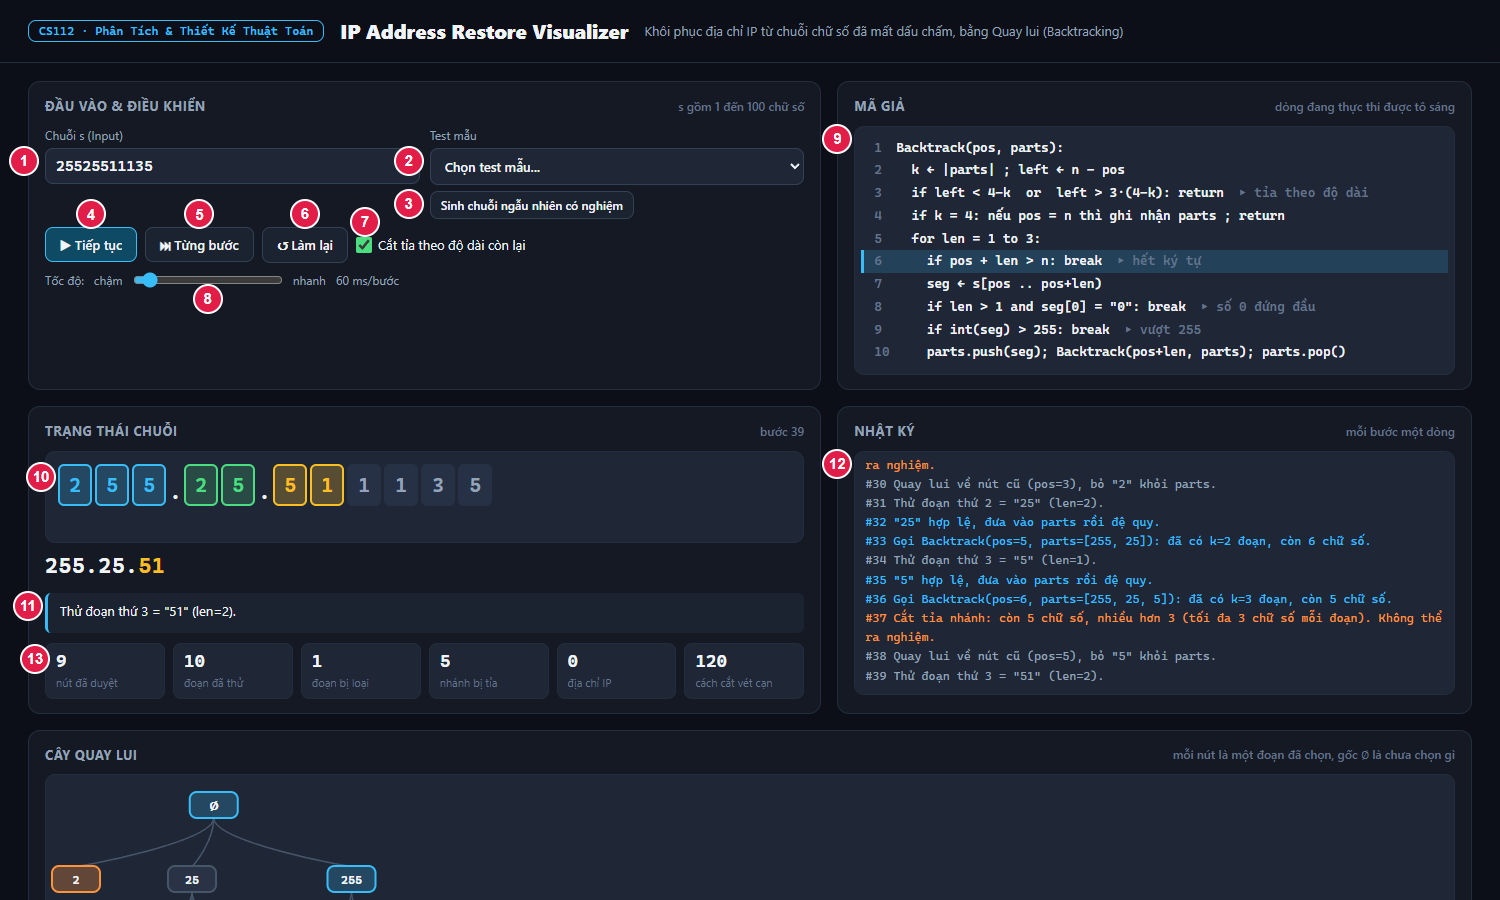
\includegraphics[width=\textwidth]{img/08_guide_top.png}
\caption{Nửa trên của bảng điều khiển (ảnh chụp lúc đang chạy dở, đã tạm dừng ở bước $39$).}\label{fig:guide_top}
\end{figure}

\textbf{Các bước dùng cơ bản.}
\begin{enumerate}
    \item Nhập chuỗi chữ số vào ô \textbf{Chuỗi s} (1), hoặc chọn một test mẫu trong danh sách (2), hoặc bấm nút sinh chuỗi ngẫu nhiên có nghiệm (3). Chuỗi hợp lệ gồm $1$ đến $100$ chữ số. Nếu nhập rỗng, có chữ cái hoặc dài quá $100$, ô nhập báo lỗi màu đỏ và các nút giải bị khóa cho đến khi sửa lại.
    \item Bấm \textbf{Bắt đầu giải} (4) để thuật toán tự chạy, hoặc \textbf{Từng bước} (5) để mỗi lần bấm là một bước. Khi đang chạy, nút (4) đổi thành \textbf{Tạm dừng}, sau khi tạm dừng đổi thành \textbf{Tiếp tục}, khi chạy xong đổi thành \textbf{Chạy lại}.
    \item Kéo thanh \textbf{Tốc độ} (8) để chỉnh thời gian giữa hai bước, từ $5$ đến $800$ ms mỗi bước. Muốn xem kỹ thì kéo về phía chậm hoặc dùng nút Từng bước.
    \item Bấm \textbf{Làm lại} (6) để xóa tiến trình và chạy lại từ đầu với chuỗi hiện tại. Sửa chuỗi trong ô nhập hoặc đổi công tắc (7) cũng tự đặt lại tiến trình.
\end{enumerate}

\textbf{Đọc các vùng hiển thị.}
\begin{itemize}
    \item \textbf{Mã giả} (9): dòng đang thực thi được tô sáng, đối chiếu với mã giả ở mục~\ref{sec:algo}. Dòng $3$ có ghi chú ``tỉa theo độ dài'', sẽ mờ đi khi tắt công tắc (7).
    \item \textbf{Trạng thái chuỗi} (10): mỗi chữ số một ô. Ô đã thuộc một đoạn được tô màu theo đoạn, ô đang thử có viền vàng (đỏ nếu đoạn bị loại). Dòng chữ lớn bên dưới là địa chỉ IP đang được xây dựng.
    \item \textbf{Dòng trạng thái} (11): một câu mô tả bước vừa thực hiện.
    \item \textbf{Nhật ký} (12): mỗi bước một dòng kèm số thứ tự và lý do. Giữ tối đa $500$ dòng gần nhất.
    \item \textbf{Sáu ô thống kê} (13): số nút đã duyệt, số đoạn đã thử, số đoạn bị loại, số nhánh bị tỉa, số địa chỉ IP tìm được, và số cách cắt mà vét cạn phải kiểm tra (để so sánh).
\end{itemize}

\begin{figure}[H]
\centering
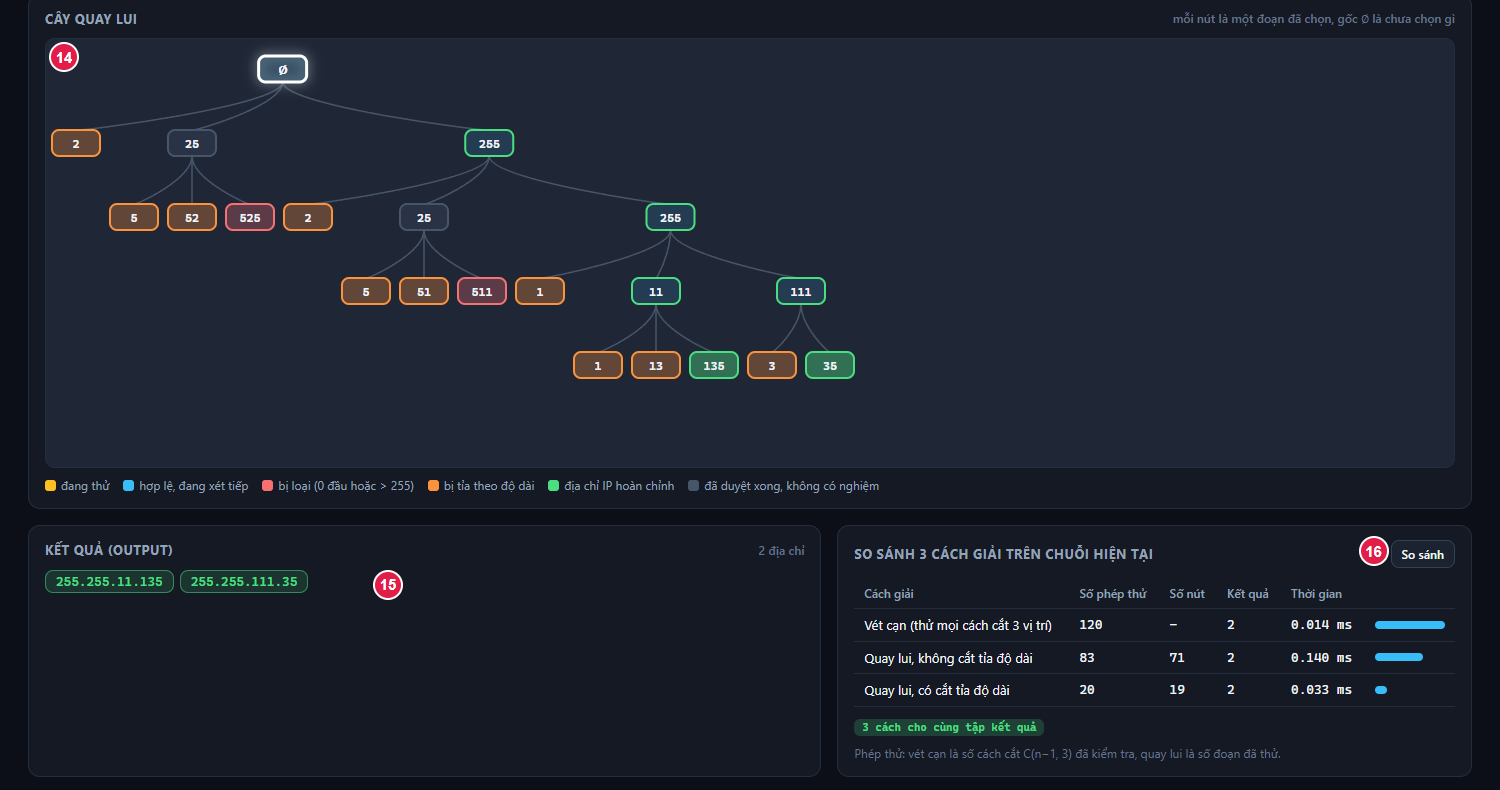
\includegraphics[width=\textwidth]{img/09_guide_bottom.png}
\caption{Nửa dưới của bảng điều khiển sau khi giải xong chuỗi \texttt{25525511135} và bấm So sánh.}\label{fig:guide_bottom}
\end{figure}

\begin{itemize}
    \item \textbf{Cây quay lui} (14): mỗi nút là một đoạn đã chọn, gốc $\varnothing$ là chưa chọn gì. Màu nút: vàng là đang thử, xanh dương là hợp lệ và đang xét tiếp, đỏ là bị loại ($0$ đứng đầu hoặc lớn hơn $255$), cam là bị tỉa theo độ dài, xanh lá là địa chỉ IP hoàn chỉnh, xám là đã duyệt xong nhưng không có nghiệm. Chú giải màu nằm ngay dưới cây.
    \item \textbf{Kết quả (Output)} (15): các địa chỉ IP tìm được, thêm dần khi thuật toán ghi nhận nghiệm.
\end{itemize}

\textbf{Các chức năng thêm.}
\begin{itemize}
    \item \textbf{Cắt tỉa theo độ dài còn lại} (7): tắt đi để thấy cây phình ra khi không tỉa, bật lại để so sánh. Đổi công tắc sẽ đặt lại tiến trình.
    \item \textbf{So sánh} (16): chạy vét cạn, quay lui không tỉa và quay lui có tỉa trên chuỗi hiện tại, hiện số phép thử, số nút, số kết quả, thời gian, và báo ``3 cách cho cùng tập kết quả'' nếu khớp nhau. Thời gian đo trong trình duyệt nên chỉ mang tính tham khảo (cỡ phần nghìn đến phần trăm mili giây với chuỗi ngắn).
    \item \textbf{Chạy toàn bộ testcase} (17): chạy quay lui có cắt tỉa trên $48$ test nhúng sẵn và so với đáp án sinh bởi vét cạn. Kết quả hiện ở dòng tổng (18) và bảng chi tiết từng test (hình \ref{fig:guide_tests}), mỗi dòng có nhóm, tên, độ dài, số đáp án, số thu được, thời gian và nhãn ĐẠT hoặc SAI.
\end{itemize}

\begin{figure}[H]
\centering
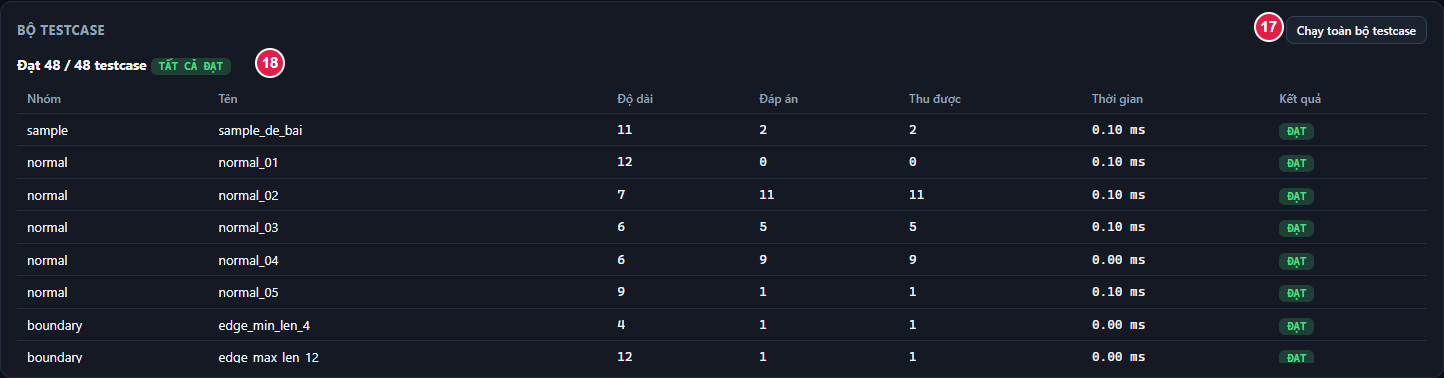
\includegraphics[width=\textwidth]{img/10_guide_tests.png}
\caption{Bảng kết quả chạy toàn bộ testcase: $48/48$ đạt.}\label{fig:guide_tests}
\end{figure}

\textbf{Một kịch bản thử nhanh (khoảng một phút).}
\begin{enumerate}
    \item Mở trang, giữ nguyên chuỗi \texttt{25525511135}, bấm \textbf{Bắt đầu giải}. Kết quả cuối cùng phải là hai địa chỉ \texttt{255.255.11.135} và \texttt{255.255.111.35}.
    \item Bấm \textbf{So sánh}. Phải thấy ba cách cùng $2$ kết quả, và quay lui có tỉa dùng ít phép thử nhất.
    \item Chọn test mẫu \textit{Có số 0 đứng đầu: 010010}, bấm \textbf{Bắt đầu giải}. Phải thấy các nút \texttt{01} và \texttt{00} màu đỏ (bị loại vì số $0$ đứng đầu), và hai kết quả \texttt{0.10.0.10}, \texttt{0.100.1.0}.
    \item Gõ \texttt{12a45}. Phải thấy báo lỗi và nút giải bị khóa.
    \item Bấm \textbf{Chạy toàn bộ testcase}. Phải thấy ``Đạt 48 / 48''.
\end{enumerate}

%=====================================================================
\section{Thiết kế thực nghiệm}

\subsection{Cách tạo testcase}
Tệp \texttt{source/gen\_testcases.py} sinh $48$ test, cố định hạt giống ngẫu nhiên (giá trị đặt ngay đầu tệp) để tái lập. \textbf{Đáp án (\texttt{.out}) không lấy từ lời giải quay lui} mà từ \texttt{ip\_bruteforce.py}, thử mọi cách cắt $3$ vị trí và kiểm tra từng đoạn. Hai cách giải hoàn toàn khác cấu trúc, nên trùng nhau là bằng chứng độc lập về tính đúng. Dòng trong \texttt{.out} được sắp xếp, khi so sánh ta cũng sắp xếp kết quả (đề cho phép thứ tự bất kỳ).

\subsection{Phân nhóm}
\begin{table}[H]
\centering
\begin{tabular}{@{}lrp{8cm}@{}}
\toprule
\textbf{Nhóm} & \textbf{Số test} & \textbf{Nội dung} \\
\midrule
sample & 1 & ví dụ của đề \\
normal & 5 & chuỗi thông thường $6$ đến $12$ ký tự \\
boundary & 9 & độ dài $1, 3, 4, 12, 13$; toàn $0$; toàn $255$; đoạn $256$ \\
special & 7 & số $0$ đứng đầu, đúng một cách, nhiều đáp án, giá trị sát $255$ \\
invalid & 2 & có chữ cái, chuỗi rỗng \\
random & 20 & $15$ test chữ số ngẫu nhiên, $5$ test chữ số $\{0,1,2,5\}$ để tăng xác suất có nghiệm \\
large & 4 & $100$ chữ số (toàn $1$, ngẫu nhiên, toàn $0$), $13$ chữ số \\
\bottomrule
\end{tabular}
\end{table}
Tổng cộng $110$ địa chỉ đáp án, một test nhiều nhất $16$ địa chỉ, $19$ test vô nghiệm (đầu vào quá ngắn, quá dài, hoặc không chia được).

\subsection{Mức độ bao phủ}
Các trường hợp quyết định của thuật toán đều có test riêng: độ dài dưới ngưỡng ($n<4$), vượt ngưỡng ($n>12$, tỉa ngay ở gốc), số $0$ đứng đầu, đoạn $>255$, đúng $255$, một nghiệm duy nhất, nhiều nghiệm. Ngoài $48$ test cố định, em còn chạy $3000$ chuỗi ngẫu nhiên (độ dài $1$ đến $14$, bảng chữ số $\{0\}$, $\{0,1\}$, $\{0,1,2,5\}$, $\{0..9\}$, $\{1,2\}$) và đối chiếu \textbf{ba} cách: quay lui, vét cạn, và module \texttt{ipaddress} của Python.

%=====================================================================
\section{Đánh giá}

\subsection{Tính đúng đắn}
\begin{itemize}
    \item $48/48$ testcase đạt, cả trong \texttt{test\_core.js} (Node.js) lẫn khi bấm ``Chạy toàn bộ testcase'' trong trang (hình \ref{fig:tests}).
    \item $3000$ chuỗi ngẫu nhiên: quay lui có tỉa, quay lui không tỉa, vét cạn cho cùng tập kết quả ($1140$ chuỗi có nghiệm). Bản Python cũng khớp \texttt{ipaddress} trên $3000$ chuỗi tương tự.
    \item Ví dụ của đề cho đúng $2$ địa chỉ.
\end{itemize}
\begin{figure}[H]
\centering
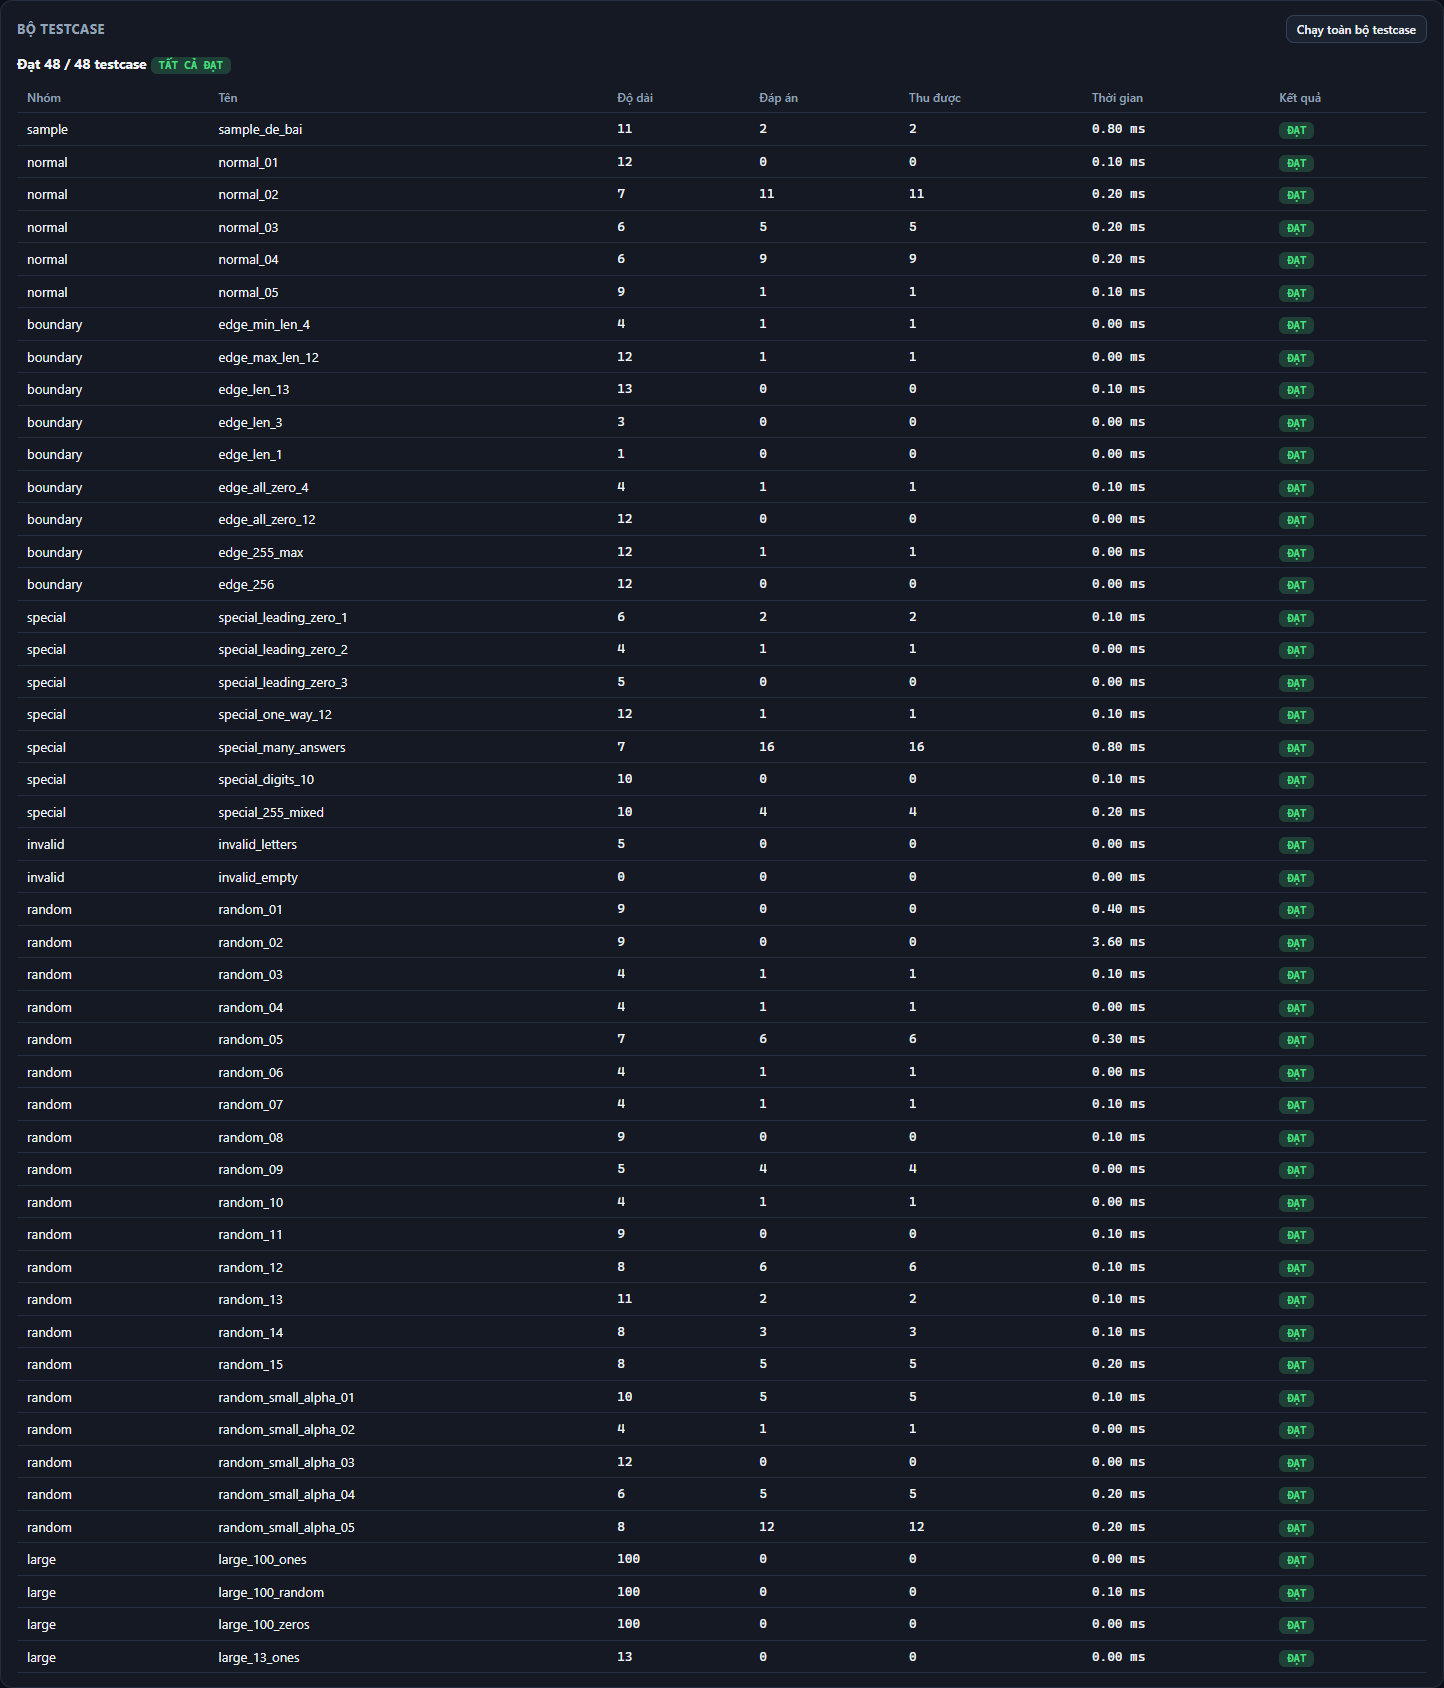
\includegraphics[width=\textwidth,max height=0.55\textheight,keepaspectratio]{img/05_tests_summary.png}
\caption{Kết quả chạy toàn bộ testcase trong ứng dụng.}\label{fig:tests}
\end{figure}

\subsection{So sánh ba cách giải}\label{sec:compare}
Số liệu do ứng dụng đo (cột ``phép thử'' là số đoạn đã thử với quay lui, và số cách cắt đã kiểm tra với vét cạn).

\begin{table}[H]
\centering
\small
\begin{tabular}{@{}lrrrrrr@{}}
\toprule
 & & & \multicolumn{3}{c}{\textbf{Phép thử}} & \\
\cmidrule(lr){4-6}
\textbf{Chuỗi} & $n$ & \textbf{IP} & Vét cạn & QL không tỉa & QL có tỉa & \textbf{Nút (có tỉa)} \\
\midrule
\texttt{25525511135} & 11 & 2 & 120 & 83 & 20 & 19 \\
\texttt{1921681}     & 7  & 11 & 20 & 60 & 56 & 51 \\
\texttt{010010}      & 6  & 2 & 10 & 16 & 16 & 13 \\
\texttt{0000}        & 4  & 1 & 1 & 7 & 7 & 5 \\
\texttt{255255255255}& 12 & 1 & 165 & 84 & 12 & 13 \\
\texttt{256256256256}& 12 & 0 & 165 & 45 & 3 & 3 \\
\texttt{1111111111111}& 13 & 0 & 220 & 120 & 0 & 1 \\
$30 \times$ \texttt{1} & 30 & 0 & 3\,654 & 120 & 0 & 1 \\
$100 \times$ \texttt{1}& 100 & 0 & 156\,849 & 120 & 0 & 1 \\
\bottomrule
\end{tabular}
\caption{Số phép thử của ba cách giải.}\label{tab:cmp}
\end{table}

\textbf{Nhận xét (kể cả điều bất lợi cho quay lui).}
\begin{itemize}
    \item Với chuỗi \emph{dài}, vét cạn tăng như $n^3$ ($156\,849$ khi $n=100$) còn quay lui chạm trần $121$ nút, và có tỉa thì chỉ $1$ nút, vì tỉa độ dài phát hiện ngay ở gốc rằng không thể có nghiệm.
    \item Với chuỗi \emph{rất ngắn}, vét cạn có thể ít phép thử hơn: \texttt{010010} (vét cạn $10$, quay lui $16$), \texttt{1921681} ($20$ so với $56$), \texttt{0000} ($1$ so với $7$). Lý do: số cách cắt $\binom{n-1}{3}$ nhỏ khi $n$ nhỏ, còn quay lui phải thử cả những đoạn sẽ bị loại. Em coi đây là kết quả thật và ghi lại, không che đi.
    \item Cắt tỉa theo độ dài chỉ có tác dụng khi chuỗi gần hoặc vượt các ngưỡng $4$ và $12$ (ví dụ \texttt{255255255255}: $84 \to 12$). Với chuỗi nằm giữa và đều hợp lệ như \texttt{1921681} ($60 \to 56$), lợi ích nhỏ.
    \item Số phép thử không phải thời gian. Đo lời giải Python $30$ lần mỗi chuỗi (tính cả khởi động trình thông dịch, khoảng $28$ ms): trung vị $57$ ms cho $n=11$, $73$ ms cho $n=12$, $83$ ms cho $n=100$, tức phần chênh so với khởi động rất nhỏ. Máy đo là Python $3.14$ trên WSL, còn bộ kiểm thử mô phỏng bộ chấm chạy bằng Python $3.12.10$ trên Windows, thời gian lâu nhất $0{,}05$ s mỗi lần. Chưa có số đo trên máy chấm thật của WeCode.
\end{itemize}

\subsection{Tính trực quan}
Mỗi bước thuật toán ứng với đúng một sự kiện trên giao diện: dòng mã giả sáng, dải chữ số đổi màu, nút mới xuất hiện trên cây, một dòng nhật ký. Có thể bấm từng bước để quan sát hoặc để chạy tự động.

\subsection{Hạn chế và hướng phát triển}
\begin{itemize}
    \item Thời gian trong bảng so sánh của ứng dụng đo bằng \texttt{performance.now()} trong trình duyệt và lặp lại tới $30$ ms, chỉ mang tính tham khảo (dao động giữa các lần chạy).
    \item Ứng dụng chỉ hỗ trợ IPv4 và chuỗi chữ số thập phân.
    \item Hướng phát triển: cho phép đặt khoảng giá trị khác $0$--$255$, hỗ trợ IPv6, hoặc đếm số nghiệm bằng quy hoạch động để so sánh với quay lui.
\end{itemize}

%=====================================================================
\section{Quy trình thực hiện với AI}

\subsection{Công cụ}
\begin{itemize}
    \item \textbf{Jcode} (trợ lý AI chạy trong terminal, có quyền đọc/ghi file và chạy lệnh), dùng một mô hình duy nhất là \textbf{Claude Sonnet 5.5} (Anthropic). Mọi công việc AI hỗ trợ trong bài này (viết code, kiểm thử, viết báo cáo) đều do mô hình này thực hiện, em không dùng mô hình ngôn ngữ nào khác.
    \item \textbf{Giọng đọc Ngọc Huyền} của engine \textbf{VieNeu-TTS} (model \texttt{VieNeu-TTS-v3-Turbo}), chạy cục bộ bằng Python đi kèm ứng dụng Reup-Video trên máy em.
    \item \textbf{Playwright} (điều khiển Chrome) và \textbf{ffmpeg} để quay và ghép video.
    \item \textbf{Tectonic} (bộ biên dịch LaTeX) để tạo PDF của báo cáo này.
\end{itemize}

\subsection{Phân công}
\begin{itemize}
    \item \textbf{Chọn bài:} em chọn bài Địa chỉ IP vì bài có liên quan tới công việc của em, và dùng quay lui theo đúng yêu cầu của đề.
    \item \textbf{AI đảm nhiệm:} viết lời giải Python, bản vét cạn, bộ sinh testcase, ứng dụng web, kịch bản video, bản nháp báo cáo này.
    \item \textbf{Em đảm nhiệm:}
    \begin{itemize}
        \item cung cấp đầu vào cho AI: yêu cầu của cô về bài tập lớn và các hình ảnh chụp liên quan tới đề tài em muốn làm (đề bài WeCode);
        \item chọn giọng đọc Ngọc Huyền cho video;
        \item xem lại kết quả của phần demo đã xây dựng;
        \item đọc lại báo cáo và điều chỉnh cho hợp lý, đầy đủ hơn;
        \item nghe lại video để kiểm tra có bị mất âm không và phụ đề có khớp với giao diện demo không.
    \end{itemize}
\end{itemize}

\subsection{Các bước và yêu cầu chính}\label{sec:testprompt}
\begin{table}[H]
\centering
\small
\begin{tabularx}{\textwidth}{@{}p{0.4cm}p{5.4cm}X@{}}
\toprule
\textbf{\#} & \textbf{Yêu cầu (tóm tắt)} & \textbf{Kết quả} \\
\midrule
1 & Em đưa đường dẫn đề bài WeCode và thư mục bài Dò Mìn cũ (để tham khảo cách tổ chức), nhờ dựng bài ``dãy IP'' có lồng giọng Ngọc Huyền. & AI kiểm tra giọng Ngọc Huyền chạy được trên máy, rồi nhờ em gửi đề bài để làm đúng đề. \\
2 & Em gửi ảnh đề bài ``Địa chỉ IP''. & Xác định đề là ``Địa chỉ IP'', bắt buộc quay lui. \\
3 & ``Làm từng cái một''. & AI viết lời giải quay lui, bản vét cạn độc lập, bộ $48$ testcase và đối chứng $3000$ chuỗi ngẫu nhiên. \\
4 & Dựng ứng dụng trực quan hóa. & AI viết \texttt{index.html}, tự kiểm thử bằng Node.js và Chrome thật. \\
5 & Làm video có giọng Ngọc Huyền. & AI viết kịch bản $11$ cảnh, sinh giọng đọc, quay bằng Playwright, ghép bằng ffmpeg. \\
6 & Viết báo cáo theo đề cô. & AI viết báo cáo này, lấy số liệu thật từ ứng dụng. \\
7 & Rà soát lại toàn bộ bằng chứng đã có, sửa chỗ nói quá. & AI lập lại todo, đối chiếu từng mục với bằng chứng, phát hiện $3$ tham chiếu mục trong báo cáo bị ghi sai số (ghi cứng, lệch so với số mục thật), và độ dài video đã lỗi thời sau khi quay lại ($2$ phút $54$ giây xuống $2$ phút $50$ giây, và sau đó là $3$ phút $9$ giây khi thêm cảnh giới thiệu các tùy chọn), sửa và biên dịch lại. \\
8 & Em đọc lại báo cáo và yêu cầu chỉnh các phần mô hình AI, lý do chọn bài, phần em đảm nhiệm, nhận xét cá nhân. & AI sửa theo yêu cầu, thêm mẫu prompt kiểm thử bên dưới. \\
9 & Rà soát điều kiện chấp nhận: kiểm tra từng yêu cầu của đề, chạy lời giải như bộ chấm, kiểm thử toàn bộ giao diện trên Chrome thật. & AI chạy $192$ lần lời giải (kiểm tra bốn dạng đầu vào) và $28$ kiểm tra giao diện, đều đạt. Phát hiện video chưa giới thiệu $3$ chức năng của ứng dụng (công tắc cắt tỉa, nút sinh chuỗi ngẫu nhiên, danh sách test mẫu) trong khi đề yêu cầu giới thiệu đầy đủ chức năng, nên thêm cảnh thứ $7$ và quay lại. \\
\bottomrule
\end{tabularx}
\end{table}

\textbf{Mẫu prompt kiểm thử đề xuất.} Đây là mẫu prompt em đề xuất dùng ngay sau khi đã cung cấp đủ đầu vào (yêu cầu của cô, đề bài, hình ảnh), để AI tự kiểm thử trước khi báo hoàn thành:
\begin{quote}
``Sau khi đã có đủ đầu vào, hãy lập plan và todo list cho toàn bộ công việc. Kiểm tra từng bước ngay khi làm xong bước đó. Viết testcase cho thuật toán và đối chiếu với một cách giải độc lập. Chạy end-to-end test trên giao diện thật (nhập input, chạy, xem output). Chỉ báo hoàn thành khi có bằng chứng (lệnh đã chạy, kết quả thấy được), và nói rõ phần nào chưa kiểm chứng được. Nếu thiếu đầu vào thì hỏi lại, không đoán.''
\end{quote}
Sau khi AI báo xong, em vẫn phải tự kiểm thử lại bằng tay (manual test) trước khi tin kết quả.

\subsection{Lỗi gặp phải và cách phát hiện, sửa}
Những lỗi dưới đây có thật, xảy ra trong quá trình làm bài này (lỗi 6 và 7 là lỗi của bản nháp báo cáo và video, các lỗi còn lại là lỗi môi trường và công cụ).
\begin{enumerate}
    \item \textbf{Cây quay lui bị cắt hàng nút cuối.} Khung vẽ cao $340$ px không đủ cho cây $5$ tầng. \emph{Phát hiện:} AI xem ảnh chụp giao diện. \emph{Sửa:} tăng lên $430$ px.
    \item \textbf{Lỗi lúc kiểm thử.} Harness Node.js khai báo trùng tên \texttt{runAll} (\texttt{SyntaxError}). \emph{Sửa:} chạy lõi thuật toán trong một \texttt{Function} riêng.
    \item \textbf{In tiếng Việt ra console Windows.} Python in lỗi \texttt{UnicodeEncodeError} vì console dùng bảng mã cp1252. \emph{Sửa:} \texttt{sys.stdout.reconfigure(encoding='utf-8')}.
    \item \textbf{Quay video báo thiếu ffmpeg.} Playwright cần bản ffmpeg riêng để ghi video. \emph{Sửa:} chạy \texttt{playwright install ffmpeg}.
    \item \textbf{Chromium của Playwright không chạy trên WSL} (thiếu thư viện \texttt{libnspr4}). \emph{Sửa:} chuyển sang dùng Chrome thật của Windows (\texttt{channel='chrome'}).
    \item \textbf{Số liệu trong báo cáo.} Bản nháp đầu của bảng ví dụ minh họa có lý do tỉa ghi sai (ví dụ nút \texttt{25.5} bị ghi ``còn $9$ ký tự'' trong khi thực tế còn $8$) và có ghi chú tự mâu thuẫn. \emph{Phát hiện:} AI tự đọc lại bảng và tính lại. \emph{Sửa:} xuất đúng cây quay lui từ ứng dụng, tính lại $k$, $\ell$ và khoảng cần có cho từng nút bằng mã, rồi thay toàn bộ bảng (mục~\ref{sec:example} và phụ lục).
    \item \textbf{Video thiếu chức năng.} Bản video đầu chưa giới thiệu công tắc cắt tỉa, nút sinh chuỗi ngẫu nhiên và danh sách test mẫu, dù đề yêu cầu giới thiệu đầy đủ chức năng. \emph{Phát hiện:} AI đối chiếu từng chức năng của ứng dụng với các thao tác trong video. \emph{Sửa:} thêm cảnh giới thiệu các tùy chọn và quay lại (video $3$ phút $9$ giây).
\end{enumerate}

\subsection{Kiểm chứng kết quả: ai làm gì}
Em tách rõ phần AI tự kiểm chứng và phần em kiểm tra, vì hai việc này khác nhau.

\textbf{AI thực hiện (em chỉ yêu cầu, không tự chạy):}
\begin{itemize}
    \item Không tin kết quả khi chưa có bằng chứng: đáp án testcase sinh bằng vét cạn, một thuật toán khác hẳn, rồi đối chiếu với chính lời giải quay lui.
    \item Chạy ba cách giải trên $3000$ chuỗi ngẫu nhiên, thêm module chuẩn \texttt{ipaddress} của Python làm cách thứ tư độc lập.
    \item Xem ảnh chụp giao diện và khung hình video, không chỉ dựa vào đầu ra của script.
\end{itemize}

\textbf{Em thực hiện:}
\begin{itemize}
    \item Xem lại hình ảnh output thông qua video demo: đối chiếu kết quả hiển thị trên giao diện (hai địa chỉ của ví dụ, bảng thống kê, kết quả $48/48$ testcase) với đáp án mẫu của đề.
    \item Đọc lại báo cáo, yêu cầu AI chỉnh các phần chưa hợp lý (mô hình AI, lý do chọn bài, phần em đảm nhiệm, nhận xét cá nhân).
    \item Nghe lại video để kiểm tra mất âm và phụ đề có khớp giao diện demo không, rồi tự kiểm thử lại bằng tay trước khi nộp.
\end{itemize}

\subsection{Nhận xét cá nhân}
AI chỉ thực sự làm tốt khi đầu vào (input) được cung cấp chuẩn và đầy đủ: yêu cầu của cô, đề bài, hình ảnh và danh sách công việc phải thực hiện. Khi đầu vào thiếu, AI dễ suy diễn rồi đưa ra kết quả sai nhưng trình bày rất tự tin, đó là hiện tượng ảo giác (hallucination). Trong bài này có hai ví dụ cụ thể: ở bản nháp đầu, bảng ví dụ minh họa trong báo cáo có lý do tỉa ghi sai, chỉ phát hiện được khi tính lại từng nút bằng mã; và bản video đầu thiếu ba chức năng của ứng dụng mà không ai nhắc, chỉ phát hiện khi đối chiếu từng chức năng với kịch bản.

Vì vậy quy trình em rút ra là:
\begin{enumerate}
    \item cung cấp đầu vào chuẩn và đủ;
    \item yêu cầu AI lập plan và todo list cho các công việc phải thực hiện;
    \item kiểm tra từng bước, viết testcase và đối chiếu với một cách giải độc lập;
    \item chạy end-to-end test khi làm xong (mẫu prompt ở mục~\ref{sec:testprompt});
    \item cuối cùng bản thân em phải kiểm thử lại bằng tay (manual test), không tin hoàn toàn vào báo cáo của AI.
\end{enumerate}

%=====================================================================
\section{Tài liệu tham khảo}\label{sec:refs}

Phần đề cung cấp cho AI không nêu luật địa chỉ IP, nên phần kiến thức này đến từ AI và được đối chiếu với các nguồn dưới đây (AI tra cứu ngày $07/10/2026$ để kiểm tra, không phải nguồn dùng để viết lần đầu).

\begin{enumerate}
    \item \textbf{WeCode, Lab\#01 (Backtracking), bài ``Địa chỉ IP''.} Đề của môn. Nguồn của tên bài, yêu cầu quay lui và ví dụ \texttt{25525511135}, lấy từ ảnh chụp đề em cung cấp.
    \item \textbf{LeetCode, 93. Restore IP Addresses.}\\ \url{https://leetcode.com/problems/restore-ip-addresses/}. Bài cùng dạng. Trang này chặn công cụ tải tự động, nên nội dung đề được đối chiếu qua bản chép trong kho \url{github.com/doocs/leetcode} trên GitHub (thư mục lời giải bài $93$). \emph{Xác nhận:} luật mỗi đoạn từ $0$ đến $255$, không có số $0$ đứng đầu, giữ nguyên thứ tự chữ số, và các ví dụ \texttt{25525511135}, \texttt{0000}. \emph{Khác đề của em:} LeetCode cho phép in theo thứ tự bất kỳ và giới hạn độ dài là $20$, còn ứng dụng này nhận đến $100$ ký tự.
    \item \textbf{RFC 3986, mục 3.2.2 (cú pháp \texttt{IPv4address}).} \url{https://www.rfc-editor.org/rfc/rfc3986}. Văn phạm \texttt{dec-octet} cho mỗi đoạn là một chữ số, hoặc hai chữ số không bắt đầu bằng $0$, hoặc ba chữ số có giá trị đến $255$. Điều này khớp với bốn ràng buộc ở mục \ref{sec:model}.
    \item \textbf{RFC 791, Internet Protocol (1981).} \url{https://www.rfc-editor.org/rfc/rfc791}. Xác nhận địa chỉ IPv4 dài cố định bốn octet ($32$ bit), tức bốn đoạn mỗi đoạn tối đa $255$. RFC này không bàn đến cách viết thập phân có chấm, nên dạng viết ``không số $0$ đứng đầu'' dựa vào RFC 3986 và LeetCode ở trên.
\end{enumerate}

\textbf{Chưa có nguồn xác nhận.} Hai điểm sau là lựa chọn của em, không có nguồn nào xác nhận cho đề WeCode: (a) thứ tự in kết quả, và (b) in rỗng khi không có địa chỉ nào hoặc đầu vào có chữ. Nếu bộ chấm của WeCode yêu cầu khác thì phải sửa lời giải. Cách cắt tỉa theo độ dài còn lại cũng gặp trong các lời giải quay lui công bố cho bài LeetCode 93, nhưng em không sao chép từ nguồn cụ thể nào, nên không ghi như một tham chiếu.

%=====================================================================
\section{Kết luận}

Em đã xây dựng ứng dụng web trực quan hóa thuật toán quay lui cho bài Địa chỉ IP: nhập chuỗi, theo dõi từng bước trên dải chữ số, mã giả, nhật ký và cây quay lui, rồi xem kết quả. Thuật toán đúng trên $48$ testcase và $3000$ chuỗi ngẫu nhiên, đối chiếu với vét cạn. Phần so sánh cho thấy quay lui có cắt tỉa thắng rõ khi chuỗi dài ($1$ nút so với $156\,849$ cách cắt cho $n=100$), nhưng không phải lúc nào cũng thắng: với chuỗi ngắn, vét cạn thử ít hơn.

\appendix
\section{Cây quay lui đầy đủ của \texttt{25525511135}}
Xuất từ ứng dụng (\texttt{runAll}, bật tỉa). Cột 1 là mã nút, cột 2 là độ sâu.
\begin{lstlisting}
 1 1 2                 tia do dai
 2 1 25                di tiep, khong co nghiem
 3 2 25.5              tia do dai
 4 2 25.52             tia do dai
 5 2 25.525            loai (>255)
 6 1 255               di tiep, co nghiem
 7 2 255.2             tia do dai
 8 2 255.25            di tiep, khong co nghiem
 9 3 255.25.5          tia do dai
10 3 255.25.51         tia do dai
11 3 255.25.511        loai (>255)
12 2 255.255           di tiep, co nghiem
13 3 255.255.1         tia do dai
14 3 255.255.11        di tiep, co nghiem
15 4 255.255.11.1      tia do dai
16 4 255.255.11.13     tia do dai
17 4 255.255.11.135    NGHIEM
18 3 255.255.111       di tiep, co nghiem
19 4 255.255.111.3     tia do dai
20 4 255.255.111.35    NGHIEM
\end{lstlisting}
Thống kê: $21$ nút (kể cả gốc), $19$ nút được duyệt, $20$ đoạn đã thử, $2$ đoạn bị loại, $10$ nhánh bị tỉa, $2$ nghiệm.

\end{document}
